
\documentclass[xcolor={dvipsnames}]{beamer}
\usepackage{amsmath}
% \usepackage{beamerthemesplit} // Activate for custom appearance
\usepackage{hyperref}
\usepackage{ragged2e}
\usepackage{amssymb}
\usepackage{verbatim}
\usepackage{lmodern}



\title{Neural Nets}
\author{Schwartz}
\date{\today}


\begin{document}

\frame{\titlepage}




{
\beamertemplatenavigationsymbolsempty
\frame{
 \frametitle{Making machines that think}
\vspace{-.75em}
{
\fontfamily{<familyname>}\selectfont
\begin{quote}
\tiny
\justify

$\;$The perceptron -- a single layer feedforward neural network -- was invented in 1957 at the Cornell Aeronautical Laboratory by Frank Rosenblatt with funding from the United States Office of Naval Research.
In a 1958 press conference organized by the US Navy, based on Rosenblatt's statements, The New York Times reported the perceptron to be ``the embryo of an electronic computer that [the Navy] expects will be able to walk, talk, see, write, reproduce itself and be conscious of its existence.''\\
\hspace{1.5em}Upon his death, the titular Reverend Thomas Bayes (1701--1761) of the renowned theorem left an unpublished manuscript deriving the distribution for the parameter of a binomial distribution. This found its way to Richard Price, who prior to posthumously reading the manuscript at the Royal Society, dutifully edited the manuscript and added an introduction that forms much of the philosophical basis for Bayesian analysis.  Mathematical historians have argued that ``by modern standards, we should refer to the Bayes-Price rule. Price discovered Bayes' work, recognized its importance, corrected it, contributed to the article, and found a use for it. The modern convention of employing Bayes' name alone is unfair but so entrenched that anything else makes little sense.'' Quite unaware of Bayes' work, the French mathematician Pierre-Simon Laplace reproduced and extended Bayes' results in 1774. It was also suggested that the blind English mathematician Nicholas Saunderson discovered the theorem some time before Bayes, but this is disputed.  \\
\hspace{1.5em}The elegant simplicity and effectiveness of Bayes' theorem for ``learning'' has prompted some psychologists to ask if the human brain itself might be a Bayesian-reasoning machine. They suggest that the Bayesian capacity to draw strong inferences from sparse data could be crucial to the way the mind perceives the world, plans actions, comprehends and learns language, reasons from correlation to causation, and even understands the goals and beliefs of other minds.  
The key to successful Bayesian reasoning is not in having an extensive, unbiased sample, which is the eternal worry of frequentists, but rather in having an appropriate ``prior''. This prior is an assumption about the way the world works. 
With the correct prior, even a single piece of data can be used to make meaningful Bayesian predictions. By contrast, 
frequentism is perhaps not well suited to making decisions on the basis of limited information -- which is something that people have to do all the time.  \\
\hspace{1.5em} It is thought by cognitive neuroscientists that neocortical development occurs in sequential layers, driven by waves of nerve growth factors which result in a self-organizating system. 
Modern so-called $\textrm{\emph{deep learning}}$ successors of the perceptron use
 Bayesian model fitting techniques to analogously sequentially train layer upon layer of neurons 
to produce \emph{unsupervised} (self-organizing) classification networks. 

%Researches have devised experiments to test if ``learning'' in the human brain copes with everyday judgments in the real world in a Bayesian manner. 

\end{quote}
}
}
}

\frame
{
 \frametitle{Objectives}

\begin{itemize}
\item understand image data
\item understand image tools and pipelines
\item understand convolutions
\item understand neural networks
\item understand how they can recapitulate other methodologies
\item understand how activating functions provides power 
\item understand how layers provide abstract feature encoding
\item understand how neural networks are trained, i.e., \\``backpropegation is gradient decent is the chain rule'' 
\item understand that backpropegation doesn't always work well
\item understand convolutional networks structure and features
\item understand there is new thing called deep learning\\
that can be viewed as an extension of neural networks
\end{itemize}

}

\frame
{
 \frametitle{Well that's interesting...}

\begin{figure}
\centering
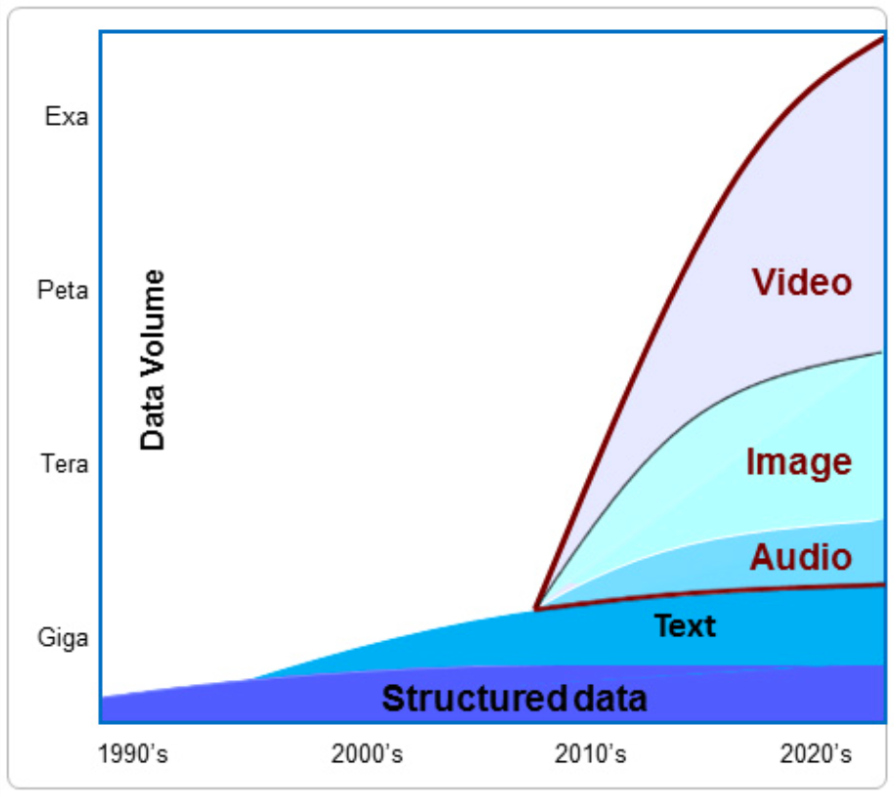
\includegraphics[width=3.5in]{image_motive.png}
\end{figure}

}


\frame
{
 \frametitle{What are images?}

\begin{figure}
\centering
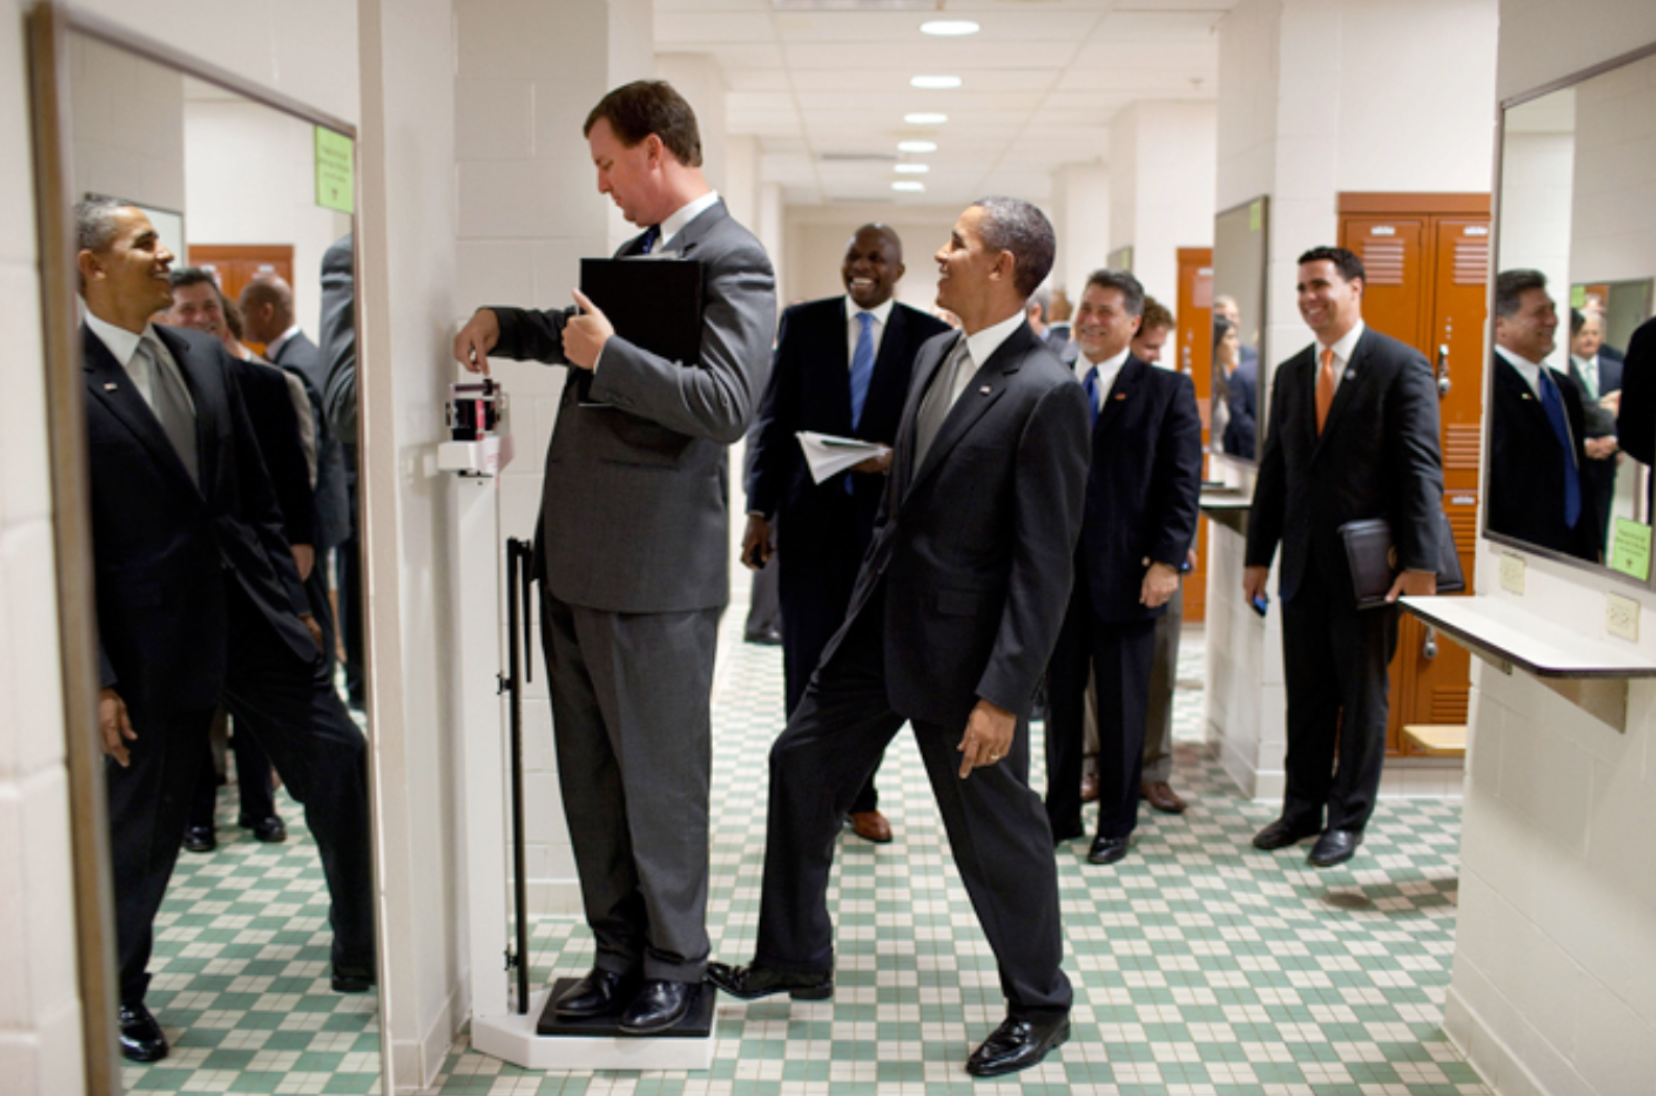
\includegraphics[width=4in]{obams.png}
\end{figure}

}

\frame
{
 \frametitle{How can computers do this??}
 
 \begin{figure}
\centering
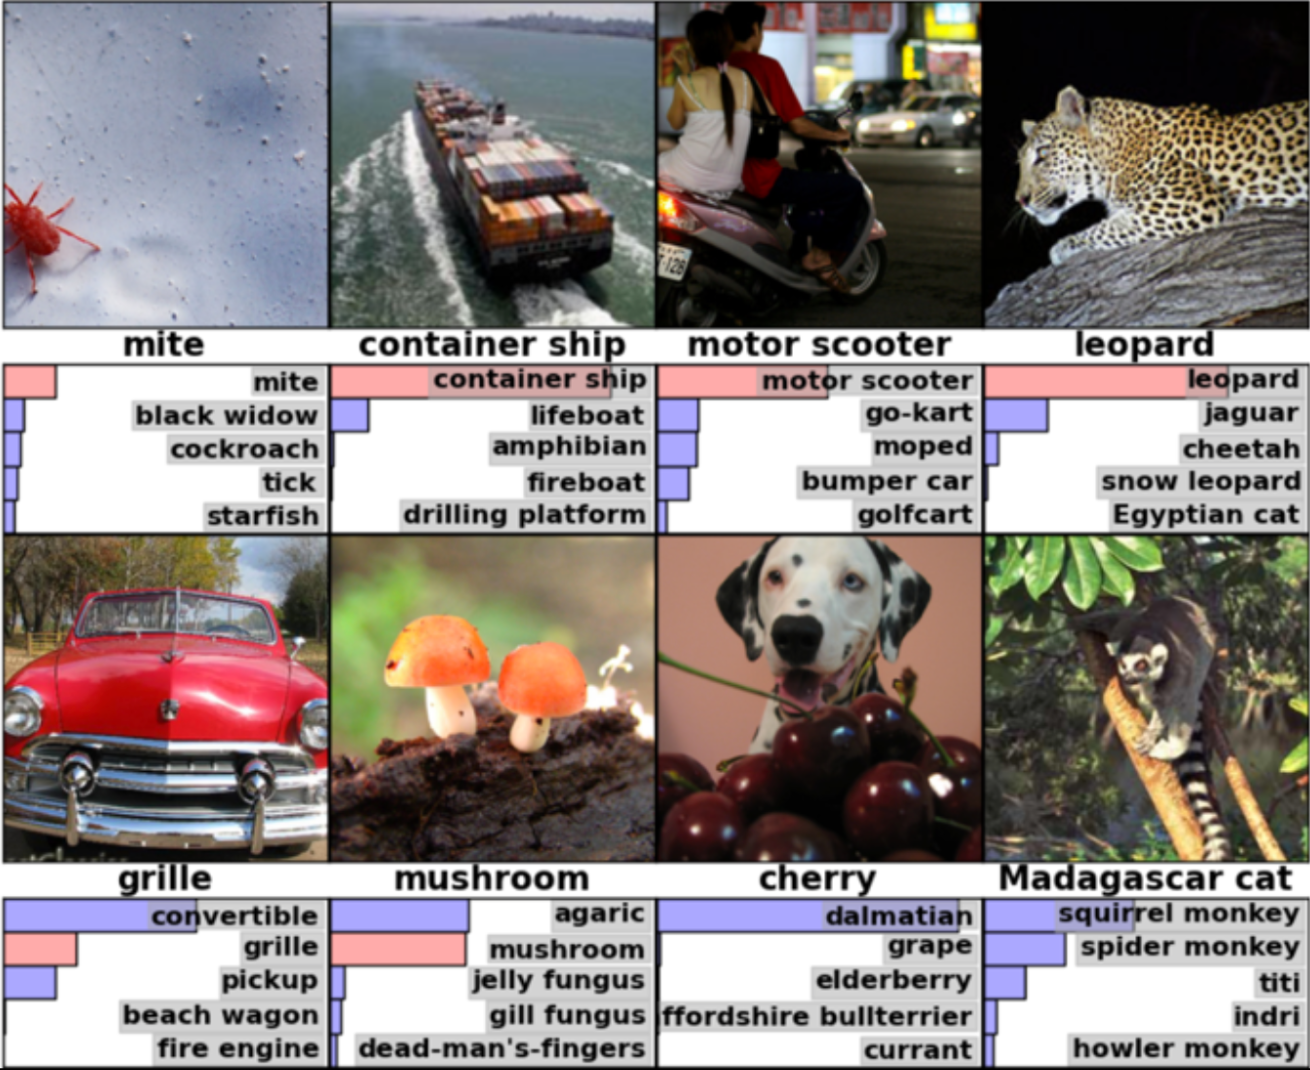
\includegraphics[width=3.5in]{pattern_rec.png}
\end{figure}

}

\frame
{
 \frametitle{How \emph{might} computers be able to do this?}
 
\Huge

 \begin{itemize}
\item<2-> Compress data
\item<2-> Keep the search simple
\item<2-> Segment image into objects
 \end{itemize}

}

\frame
{
 \frametitle{Image processing \emph{tasks}}
 
 \newcommand{\rgb}{\textcolor{red}{R}\textcolor{green}{G}\textcolor{blue}{B}}
 
\begin{itemize}
\item Read


\onslide<2->{./dog\_cat  \\./dog\_cat/dog $\;$  ./dog\_cat/cat \\
\begin{figure}
\centering
\LARGE
$\bigg[\bigg[$\raisebox{-.9em}{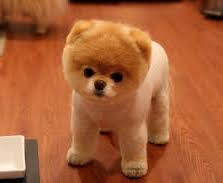
\includegraphics[height=.5in]{dog1.jpg}$,$} \raisebox{-.9em}{
\includegraphics[height=.5in]{dog2.jpg}$,$} \raisebox{-.9em}{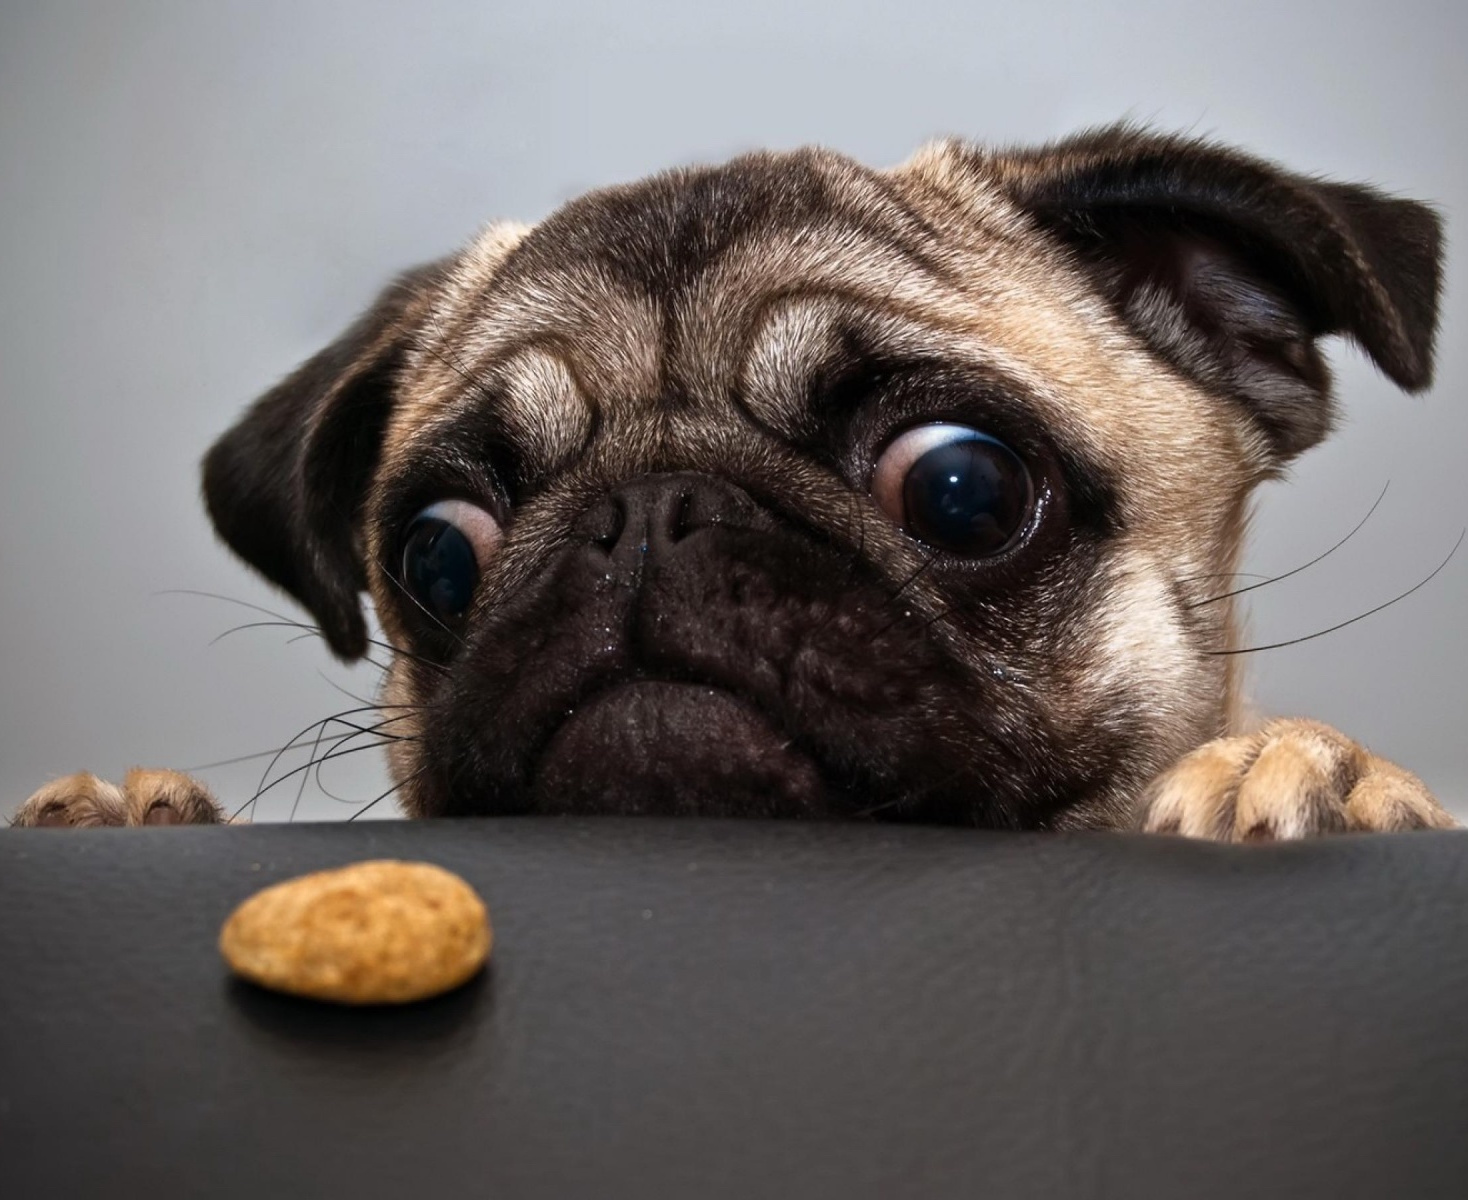
\includegraphics[height=.5in]{dog3.jpg}}$\bigg]_,$\\
$\bigg[$\raisebox{-.9em}{
\includegraphics[height=.5in]{cat1.jpg}$,$} \raisebox{-.9em}{
\includegraphics[height=.5in]{cat2.jpg}$,$} \raisebox{-.9em}{
\includegraphics[height=.5in]{cat3.jpg}}$\bigg]\bigg]$
\end{figure}
}
\normalsize

\item[] 
\item<3-> image.shape = (width, height) or (width, height,3)
\item[]<4-> A \emph{tensor} (e.g., a color image) is a matrix of vectors
$$\left[\begin{array}{cccc} \rgb &\rgb &\cdots & \rgb\\ \rgb &\rgb &\cdots & \rgb\\ \vdots & \vdots & \ddots &\vdots \\ \rgb &\rgb &\cdots & \rgb\\\end{array}\right]$$
 \end{itemize}

}


\frame
{
 \frametitle{Image processing \emph{tasks}}
 
\begin{itemize}
\item Resize \onslide<2->{\textcolor{gray}{to create a uniform feature set}}
\item[]<3-> Down/Upsampling -- \emph{not cropping} -- bi-linear interpolation
\vspace{-1.25em}
\begin{columns}
\begin{column}{.4\textwidth}
%\vspace{1.25em}
\begin{figure}
\centering
\fbox{
\includegraphics[width=1.75in]{down.png}}\\

\fbox{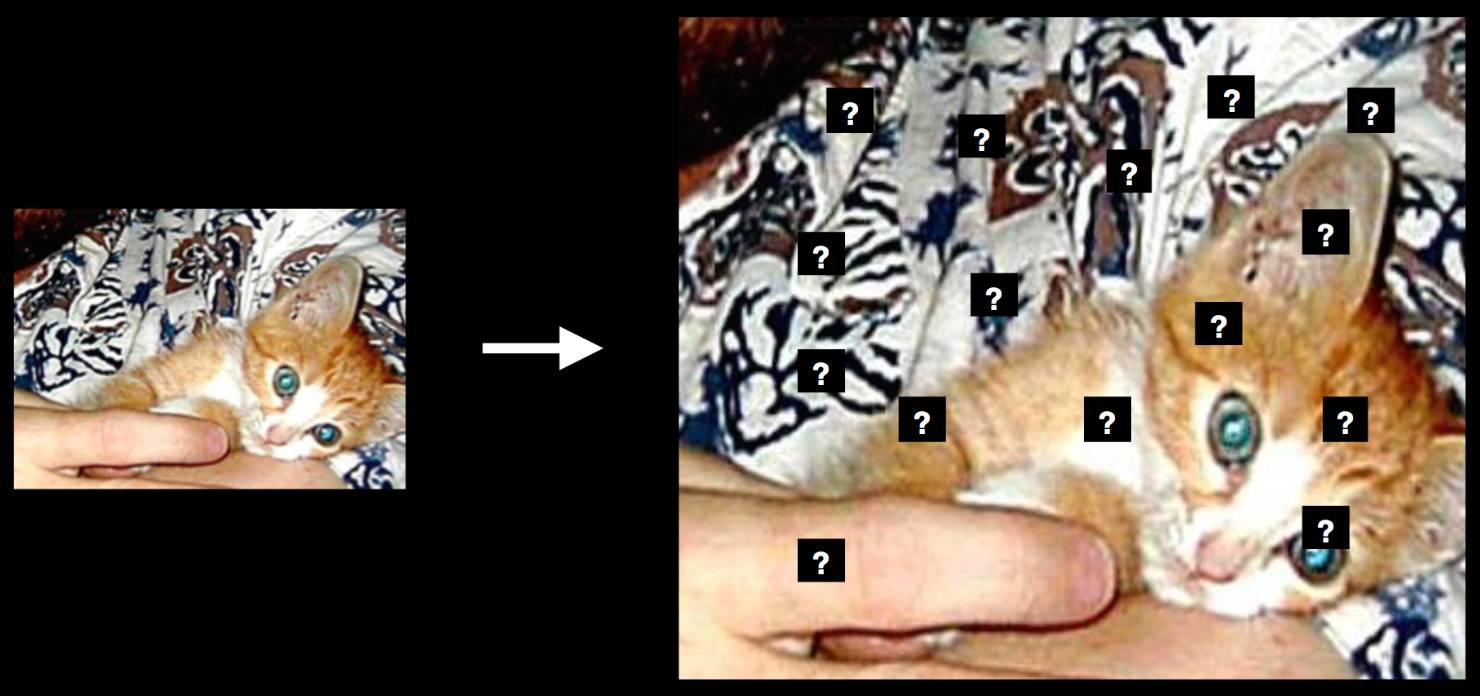
\includegraphics[width=1.75in]{up.png}}
\end{figure}

\end{column}
\begin{column}{.5\textwidth}
\begin{figure}
\centering
\fbox{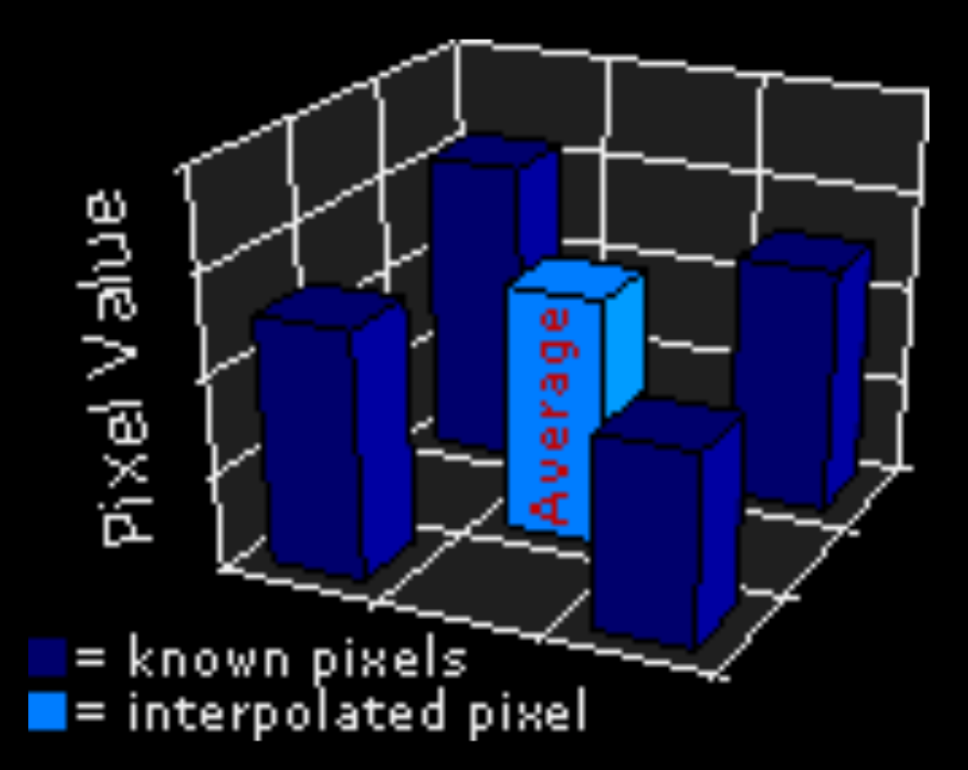
\includegraphics[width=2.3in]{interp.png}}
\end{figure}
\end{column}
\end{columns}

\item[]
\item[]<4-> Reduce size/processing time
\item[]<5-> Resolution visually checkable
 \end{itemize}
}



\frame
{
 \frametitle{Image processing \emph{tasks}}
 
\begin{itemize}
\item Denoise: remove unnecessary details to allow for \& better\\
 \textcolor{white}{Denoise:} generalization of images to image classes\\
\end{itemize}

\begin{figure}
\centering
{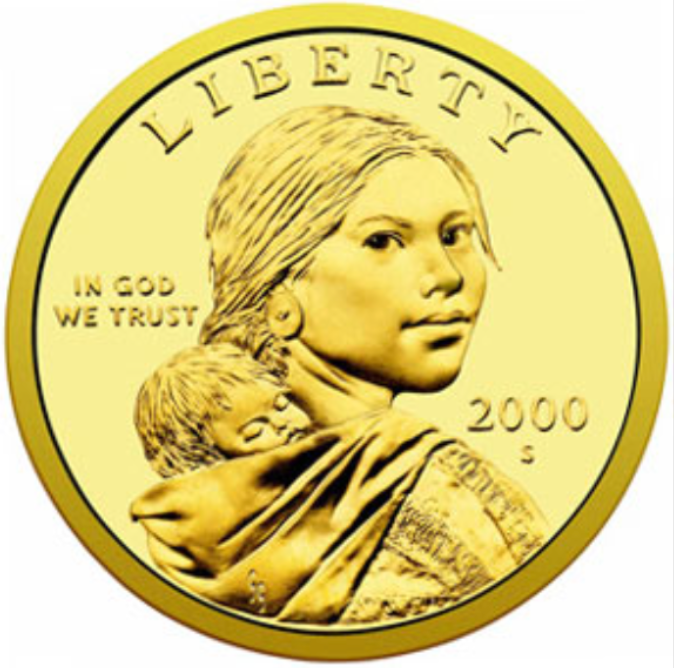
\includegraphics[width=1.75in]{dn1.png}}$\;\;${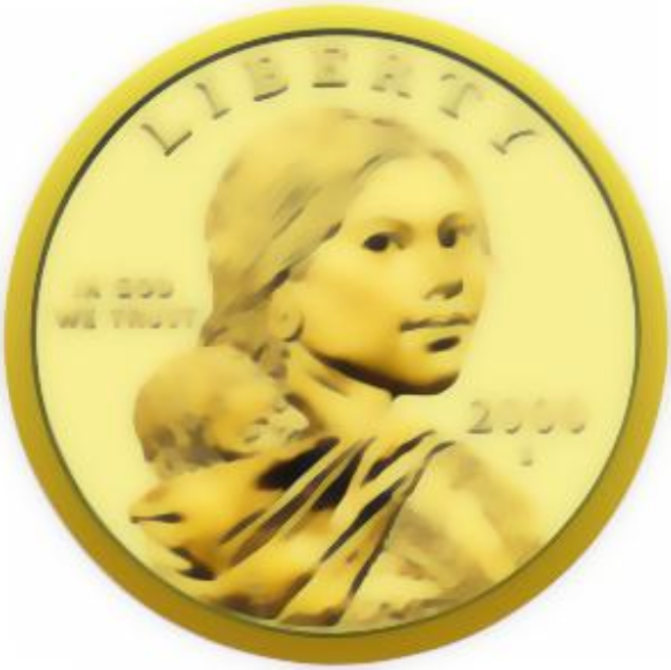
\includegraphics[width=1.75in]{dn2.png}}
\end{figure}

}


\frame
{
 \frametitle{Image processing \emph{tasks} -- more on denoising}
 
\begin{itemize}
\item<1-> Spatial proximity \emph{and pixel agreement (bi-lateral)}

\begin{figure}
\centering
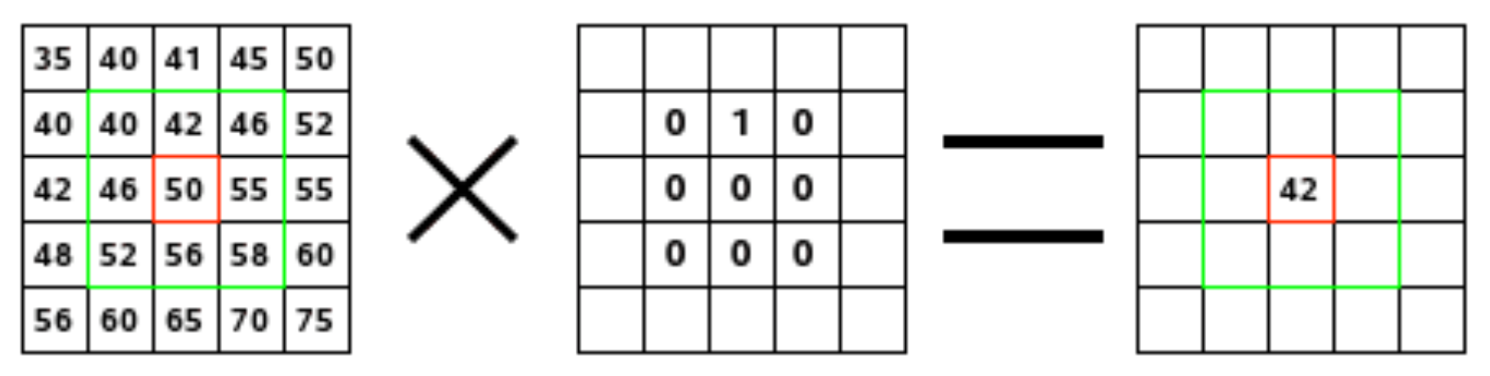
\includegraphics[height=.75in]{convolution.png}\\${}$\\${}$\\
\vspace{-.075in}
\onslide<2>{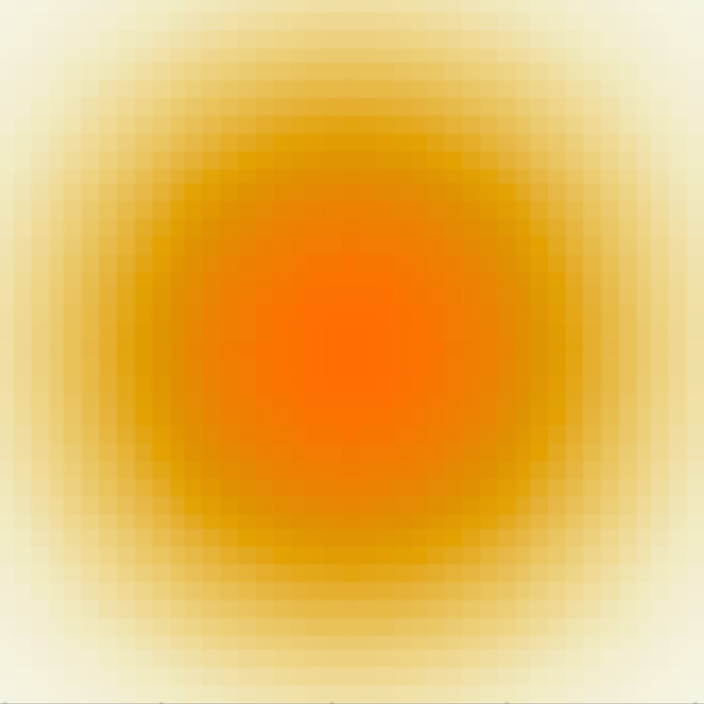
\includegraphics[height=.675in]{gaussian_convo.png}}

\vspace{-.95in}
\onslide<3>{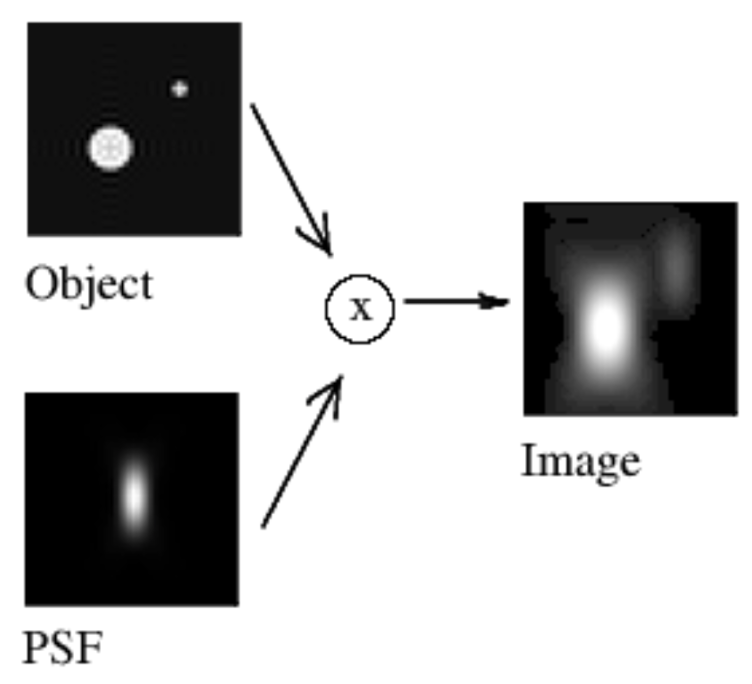
\includegraphics[height=2.1in]{convo2.png}\textcolor{white}{..-..-..-..-.--..}}


\vspace{-2in}
\onslide<4->{\fbox{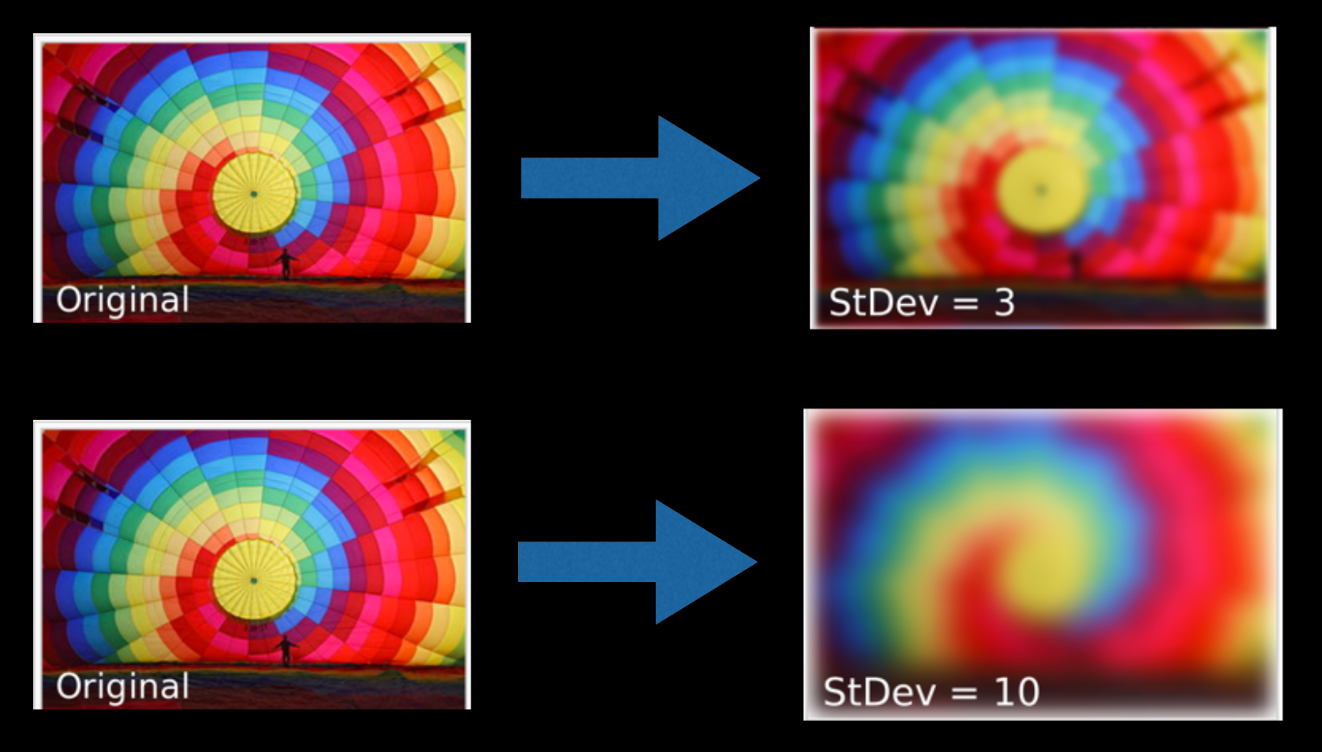
\includegraphics[width=2.9in]{smosh.png}}}

\end{figure}

\end{itemize}

}

\frame
{
 \frametitle{Image processing \emph{tasks} -- more on denoising}
 
\begin{itemize}
\item Variation Minimization: Variation Fidelity tradeoff

$$ x_i \rightarrow y_i : \underset{\boldsymbol y}{\text{min}} \quad \underset{Fidelity}{\frac{1}{2}\sum(x_i -y_i)^2} + \lambda \underset{Variation}{\sum |y_{i+1}-y_i|}$$
\end{itemize}

\onslide<2->{$$\textcolor{gray}{\text{[What is a ``hard'' image for this procedure?]}}$$}

}



\frame
{
 \frametitle{Image processing \emph{tasks}}
 
\begin{itemize}
\item<1-> Grayscale (luminescence): Tensor $\rightarrow$ Matrix
$$\text{Normalize } 0.2125\textcolor{red}{R} + 0.7154  \textcolor{green}{G} + 0.0721 \textcolor{blue}{B}$$ 
\item<2-> Edge detection (grayscale): detects large pixel transitions
\end{itemize}
\onslide<2->{\begin{figure}
\centering
{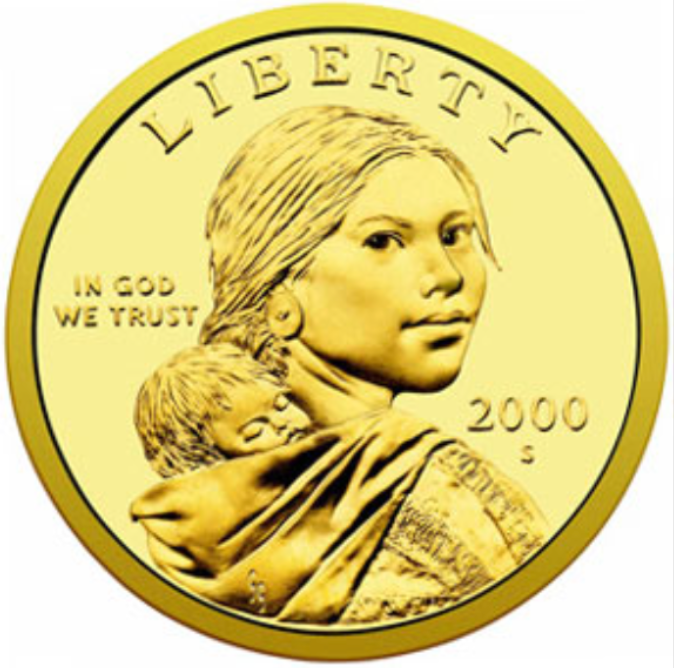
\includegraphics[width=1.25in]{dn1.png}}$\;${
\includegraphics[width=1.25in]{dn3.png}},{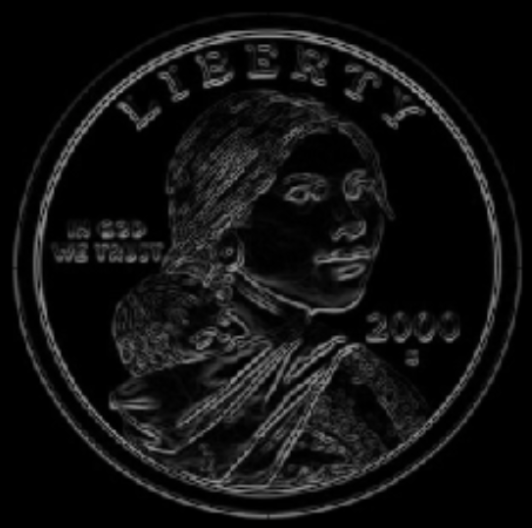
\includegraphics[width=1.25in]{dn4.png}}
\end{figure}}

}


\frame
{
 \frametitle{Image processing \emph{tasks} -- more on edge-detection}

It may be easier to identify objects if we just consider the edges


\begin{figure}
\centering
\fbox{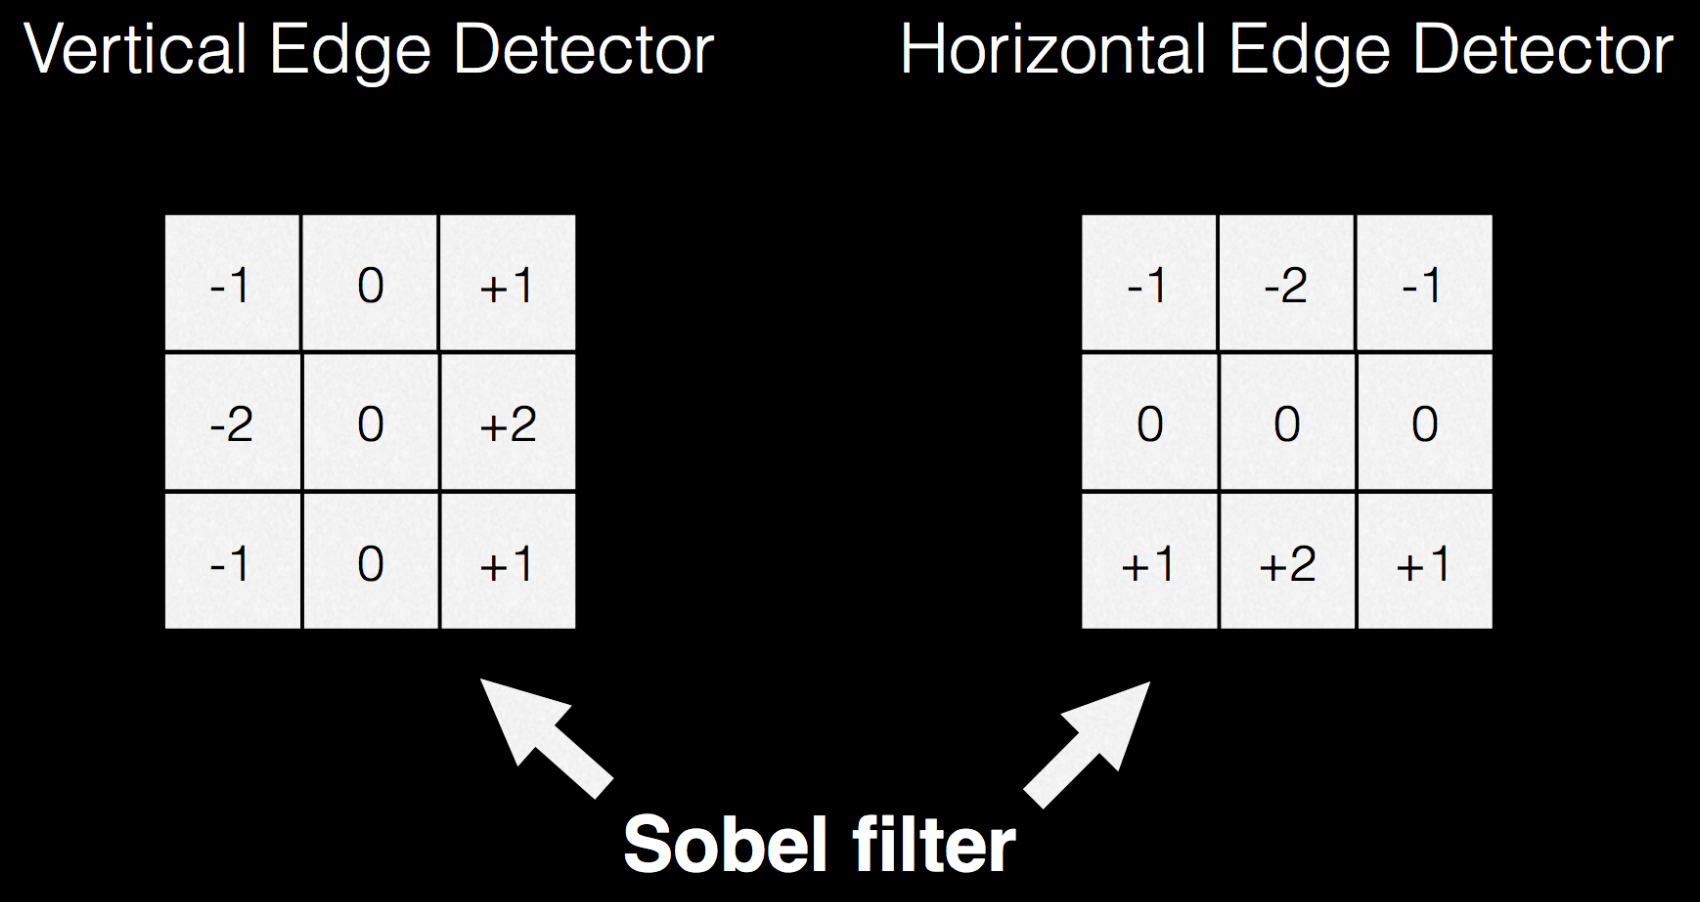
\includegraphics[height=1.12in]{convol2.png}} \fbox{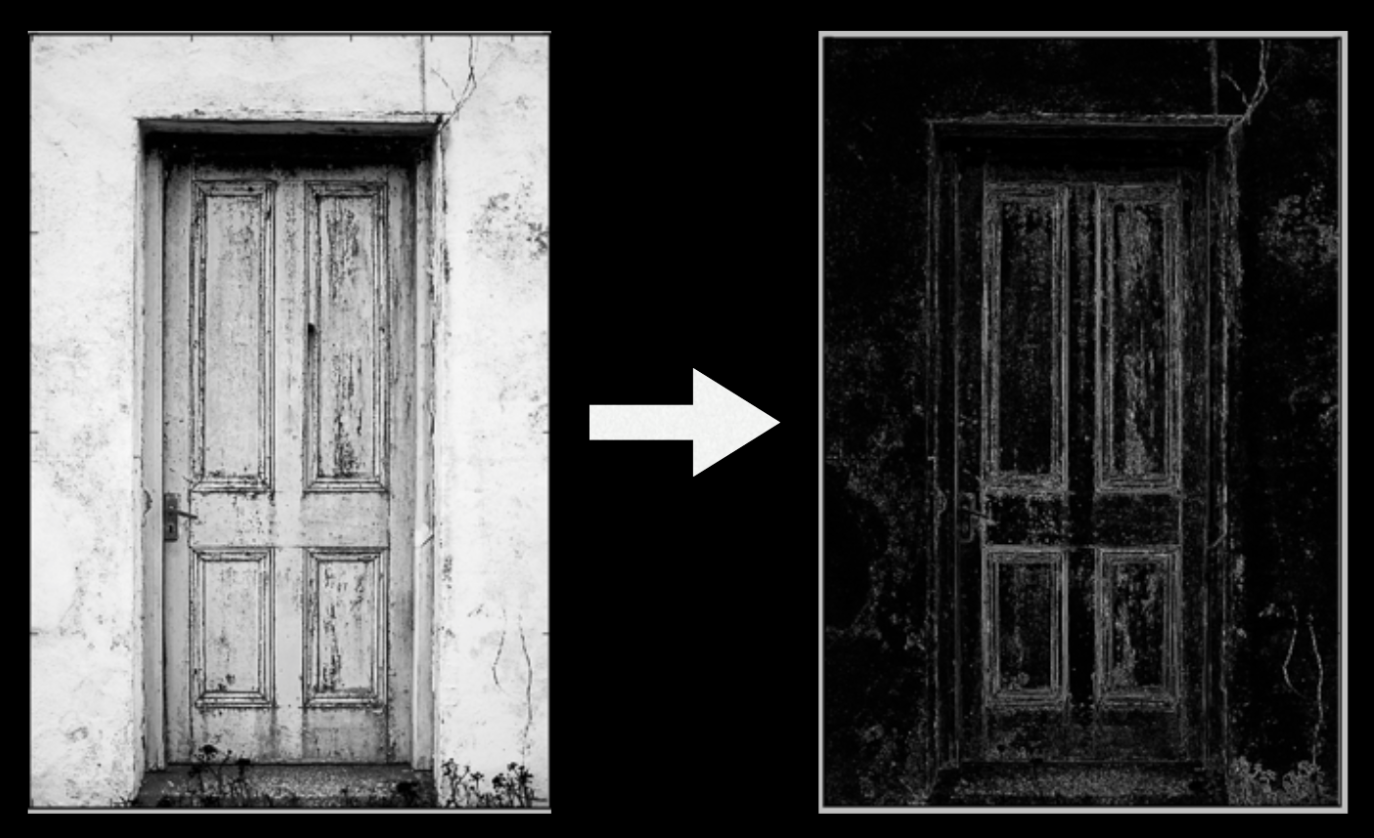
\includegraphics[height=1.12in]{convol3.png}}
\end{figure}

We may be able to use intensity gradients for feature ascertainment

\begin{figure}
\centering
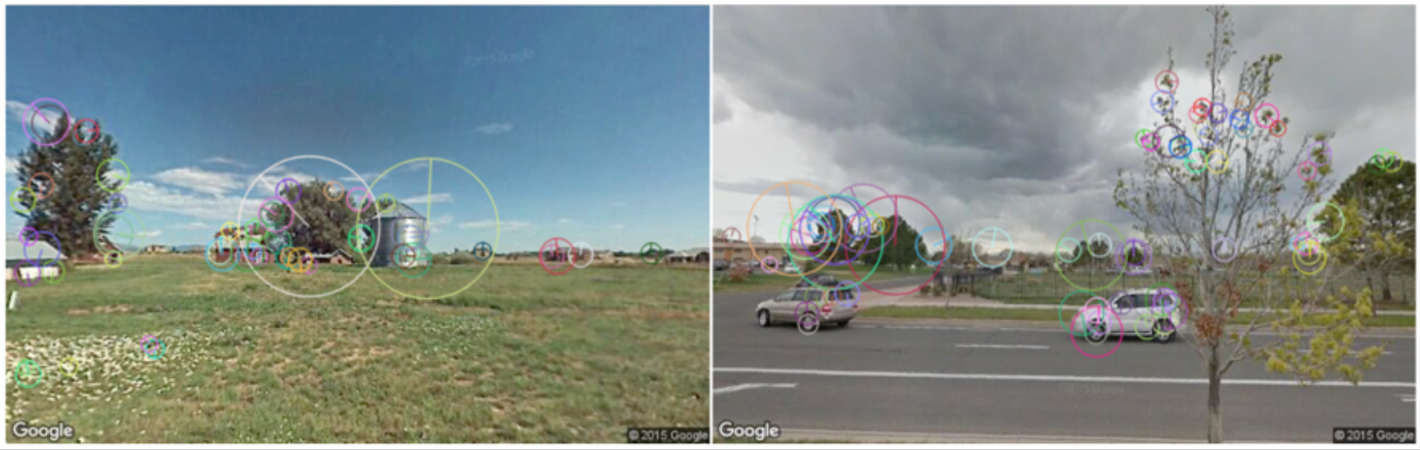
\includegraphics[height=1.3in]{intgrad.png}
\end{figure}

}




\frame
{
 \frametitle{Image processing \emph{tasks}}

\begin{itemize}
\item Image processing libraries 
 \begin{itemize}
\item Scikit-image (skimage)
\item OpenCV (and dependencies) 
\item Python Imaging Library
\item Pillow (a fork of the above)
\item etc. 
 \end{itemize}
\end{itemize} 
}




\frame
{
 \frametitle{Image \emph{Color Structure}}
 
\begin{figure}
\centering
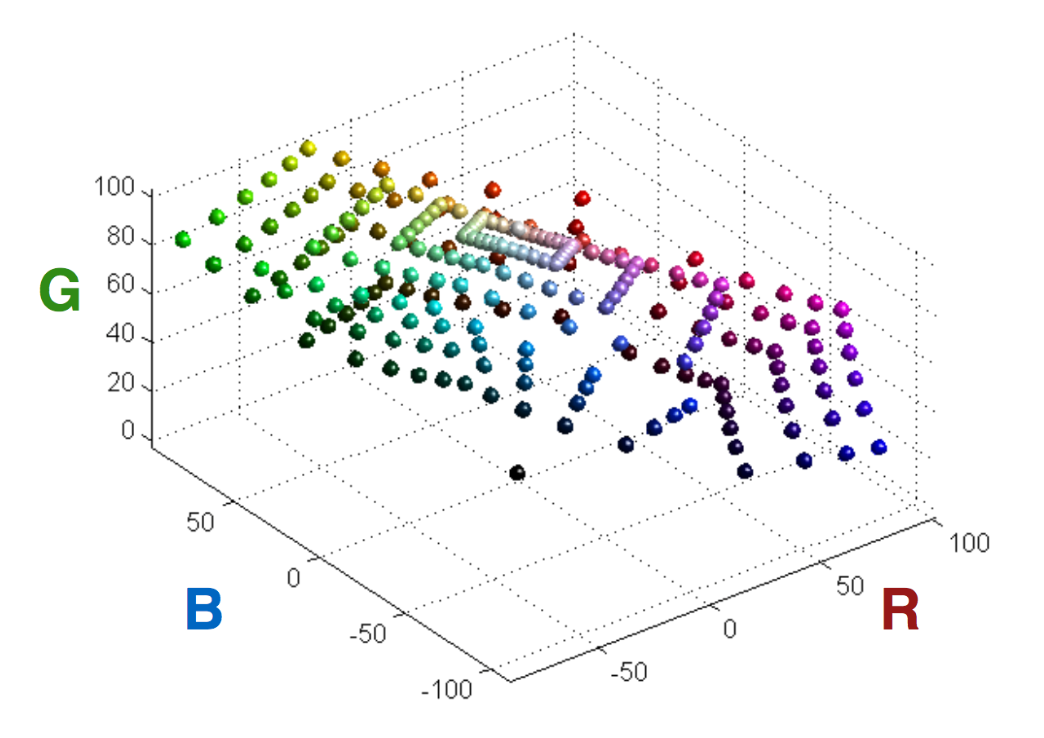
\includegraphics[height=2.25in]{rgeebee.png}
\end{figure}
}

\frame
{
 \frametitle{Image \emph{Color Structure}}
 
\begin{figure}
\centering
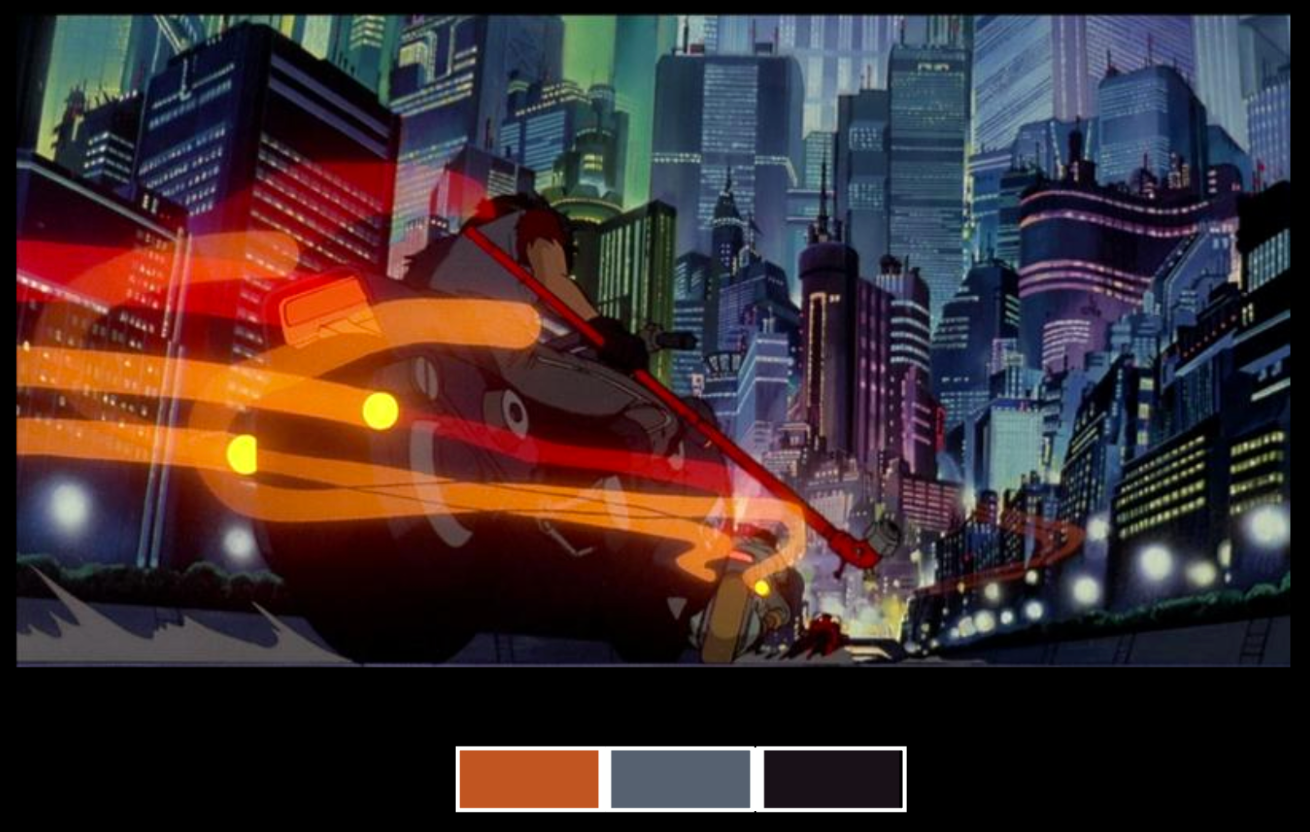
\includegraphics[height=2.25in]{cool.png}
\end{figure}
}


\frame
{
 \frametitle{Image \emph{Featurization}}

\begin{figure}
\centering
\fbox{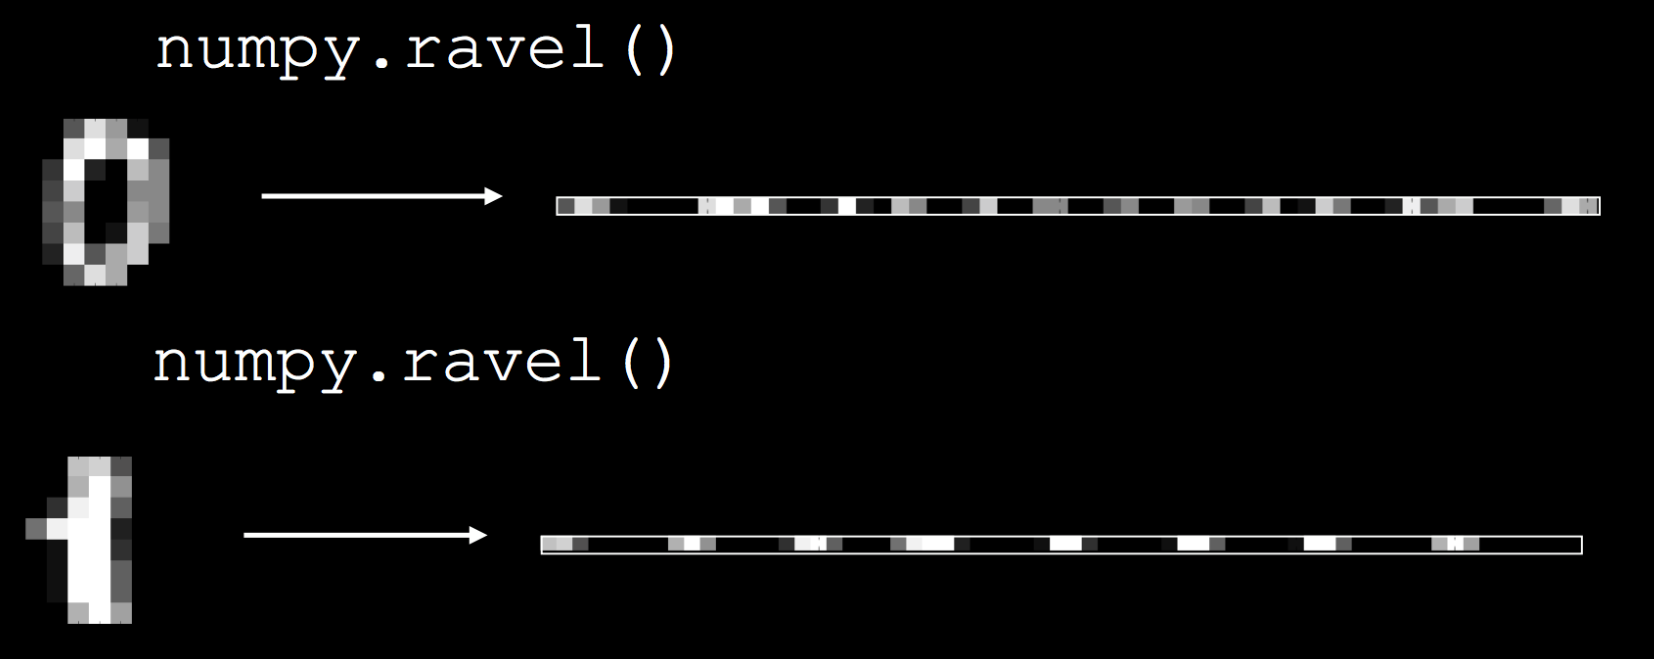
\includegraphics[width=3.75in]{vectorize.png}}
\end{figure}

}



\end{document}


\frame
{
 \frametitle{Some more convolutions}

I'm showing you these things and you are asking me:\\
``Scott -- no, the other Scott -- why are we doing this?''\\${}$\\

And I am not telling you.
}

